
\chapter{Vectors}

\index{vector}
As I stated on p.~\pageref{mathematicalObject}, every ``algebra'' is comprised
of a set of mathematical objects which you can combine with various operations.
In linear algebra, those building blocks are \textbf{vector}s and
\textbf{matrices} (singular: matrix). Buried within them are many mysteries.
We'll cover them in considerable detail in this chapter and the next.

\section{Vector vs.~scalar quantities}

\index{scalar}
\index{scale of measure}

The first thing we should do is perhaps distinguish between a vector quantity
and a \textbf{scalar quantity}, which probably had the spotlight in most of
your previous math classes. A scalar value is simply a \textit{single} number,
like 5, or -3.2, or $\pi$, or even $9 + 2i$ if you're into imaginary numbers.
The word \textit{scalar} is related to the word \textit{scale}, as in a ``scale
of measure.'' Think of stepping on a scale to weigh yourself in the morning:
your scale gives you back a single number (which you may or may not like; I
won't judge).

\index{one-dimensional quantity}
\index{dimension}

We'll call scalars \textbf{one-dimensional} values. That might seem odd, since
we haven't really talked about ``dimensions,'' yet. But think of the plain-old
\textbf{number line} you learned about back in elementary school. Zero's drawn
in the middle, positive numbers to the right and negative numbers to the left,
and the whole thing extends infinitely in just one direction\footnote{It might
seem like ``two directions,'' since the number line goes both to the left and
to the right. But since \index{left-ness} \index{right-neww} left-ness is the
exact opposite of right-ness, these are considered ``the same direction''; it's
just a matter of how far you go back or forth you go along that one straight
path.}.

% TODO: draw number line

\index{tuna fish}
\index{stock price}

Examples are so ubiquitous they're hardly worth mentioning. A person's weight
in the morning is a scalar. A company's stock price on a given day is a scalar.
So is the net \textit{movement} (up or down) of a stock's price from one day to
the next. So is a respondent's answer to the survey question ``on a 1-to-10
scale, how much do you enjoy tuna fish?'' You can think of countless others.

We of course often use variables to represent scalar quantities, and in this
book we'll put a variable in italics (like ``\textit{x}'' or
``\textit{price}'') to signify that its underlying value is a scalar quantity.

\subsection{A vector: a multi-dimensional quantity}
\index{vector}

Now a vector quantity is kind of the same thing, except that it represents
\textit{more than one} value. Suppose we wanted to represent not just a stock's
price on a given day, but an entire year's worth of prices on consecutive days.
Then, we would need a vector quantity. Instead of a survey respondent's answer
to just one question, we might want to store her entire set of answers to all
twenty questions on the survey. Instead of tracking just my weight, I might
want to record my weight, height, BMI (body-mass index), and pulse, all at a
given moment.

\index{losing information}
\index{information loss}

Vectors are \textbf{multi-dimensional} quantities. And they can't be
represented on a number line. Let's say my weight is 210 lbs.~and my height is
6'2", or 74 inches. (This is not theoretical.) I could of course draw a number
line and put a dot at 74 and another dot at 210, but this wouldn't fully
represent the fact that my weight was 210 and my height was 74. For one thing,
the numbers are on completely different scales. (There's that word ``scale''
again.) For another, it's not clear which is which -- is the right-most point
supposed to be my height, or my weight? Trying to squeeze a two-dimensional
quantity into a one-dimensional number line would \textbf{lose information.}
We need a representation scheme that can accommodate the complexity of our
quantity.

\index{Cartesian plane}
\index{coordinate plane}

For a two-dimensional quantity like weight-and-height, the obvious choice is
the two-dimensional Cartesian plane. I've drawn the vector with my height and
weight on the left side of Figure~\ref{fig:vector}. You'll see that there's an
\textit{arrow} from the origin to the point (210,74), rather than just a
circular dot at that point, as you might have expected. This is because
sometimes, it turns out, we want to treat a vector as ``a net movement in a
particular direction for a particular distance.''


\begin{figure}[ht]
\centering
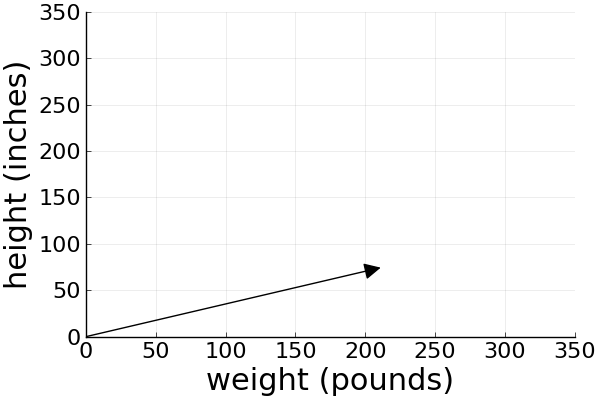
\includegraphics[width=0.4\textwidth]{vector.png}
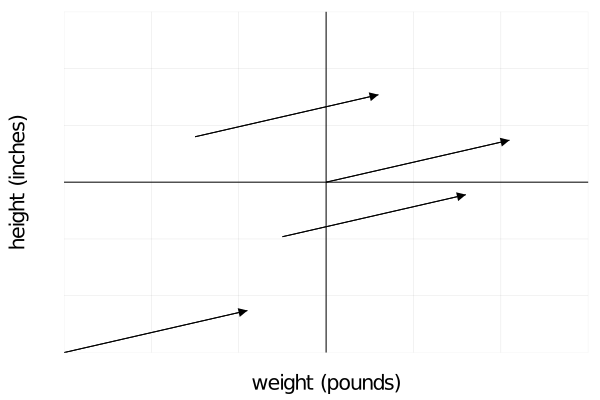
\includegraphics[width=0.58\textwidth]{vectors.png}
\caption{Left: a two-dimensional vector, depicted in a Cartesian plane. Right:
several copies of \textit{the same vector}, shown originating at various
points. They're considered ``the same'' vector because they all go in the same
direction and have the same length; the point they start at is irrelevant.}
\label{fig:vector}
\end{figure}

You can see this illustrated on the right-hand side figure, where I've drawn
several copies of \textit{the same vector}. This may seem weird, but in terms
of pictures, here's how you want to think of it: \textbf{a vector has a
direction and a length, but not a starting point}. In the case of Stephen's
biometrics, the vector's direction is east-by-northeast-ish (19.4\textdegree\
to be exact, if you wanted to work out the trig) and its length is 222.6
(Pythagorean Theorem), but it doesn't have an intrinsic ``starting point'';
it's just an arrow pointing this-a-way and yea-far, no matter where it's
anchored.

\index{mosquito}

Interestingly, the word \textit{vector} comes from a root meaning ``to carry.''
You may have heard people describe mosquitoes as being ``vectors'' for a
particular disease -- this means that they carry that disease. By thinking of a
vector as an arrow like in Figure~\ref{fig:vector}, the ``carry''
interpretation might start to make sense. A vector can represent a
transposition from one point to another. If I grew 74 inches taller and gained
210 more pounds, my point on the Cartesian plane would move in the direction
and the distance of that arrow.

\subsection{Don't visualize this}

Now that was all for \textit{two} dimensions. What about vectors with three, or
five, or even twenty dimensions? Well, for the three-dimensional case you can
indeed draw a 3-d figure with three axes, and plot three-dimensional points on
it. It turns out that most humans, though, are positively horrible at
interpreting such plots. And when you move beyond three dimensions, it's
utterly hopeless. (A friend of mine in fourth grade claimed he could visualize
four dimensions in his head, but I didn't believe him and still don't.)

But importantly, that doesn't mean we won't ever deal with higher-dimensional
vectors. In fact, vectors with lots and lots of dimensions will come up
constantly for us in this book -- believe it or not, we'll do an example where
the vectors have 50,000 dimensions! :-O

Don't worry; this won't make your head explode. In fact, it's a lot easier than
you might think to work with very high-dimensional vectors. Consider the
example I gave above about tracking a company's stock price every day for a
year. That's just a list of 365 numbers, all in a row. How hard is that to
imagine?

To work with vectors of more than three dimensions, you only have to do one
thing: give up trying to visualize them in a geometric space. As I'll describe
in the next section, it only occasionally makes sense to think about vectors
geometrically anyway; much of the time, we'll simply think of them as
quantities that have more than one component, unlike their simple brethren the
scalars.

\smallskip

Finally, the notation we'll use for vector variables. Instead of putting the
variable name in italics, we'll put it in bold-face with an arrow on the top of
it, like this: $\overrightarrow{\textbf{x}}$. The individual components of the
vector will be listed in boxies (square-brackets) like this: $[\ -2\ \ 5.9\ \
17\ \ -3\ ]$. So, if we define $\overrightarrow{\textbf{stephen}}$ as the
vector with my height and weight in it, we would write:

\vspace{-.15in}

\begin{align*}
\overrightarrow{\textbf{stephen}} = [\ 210\ \ 74 \ ].
\end{align*}



-----


5 different ways to think about a vector

1. a 2-d vector of reals, w/ index  (index into the X vector and get a value,
which is the element)
2. higher than 2 dimensions. can't visualize it; have to suspend our disbelief.
3. names instead of indices  (even less geometric)
4. non-numeric elements
5. a thing that satisfies certain properties
